\documentclass[11pt, a4paper]{article}
\usepackage[utf8]{inputenc}
\usepackage[T1]{fontenc}
\usepackage[hmargin=15mm, tmargin=25mm, bmargin=25mm]{geometry}
\usepackage[english, main=ngerman]{babel}
\usepackage{fancyhdr}
\usepackage{titlesec}
\usepackage[table]{xcolor}

\usepackage{enumitem} %needed to change enumerate options
\usepackage{graphicx}
\usepackage{amsfonts, amsmath, amssymb}
\usepackage{tabularx}
\usepackage{ragged2e}
\usepackage{xltabular}
\usepackage{rotating}

\usepackage{amsmath}
\usepackage{tikz}
\usepackage{color}

\usepackage{amsmath}
\usepackage{tikz}
\usepackage{color}
\definecolor{boxColor}{RGB}{192 192 192}
\definecolor{plusColor}{RGB}{48 191 48}
\definecolor{minusColor}{HTML}{be0105}
\newcommand\tab[1][1em]{\hspace*{#1}}

\newcommand{\myPlus}{\ \fcolorbox{black}{boxColor}{\color{plusColor}$\boldsymbol{\pmb{+}}$}\ }
\newcommand{\myPlusblank}{\ \fcolorbox{black}{white}{\color{plusColor}$\boldsymbol{\pmb{+}}$}\ }
\newcommand{\myMinus}{\ \fcolorbox{black}{boxColor}{\color{minusColor}$\boldsymbol{\pmb{-}}$}\ }
\newcommand{\myMinusblank}{\ \fcolorbox{black}{white}{\color{minusColor}$\boldsymbol{\pmb{-}}$}\ }
\newcommand{\myBox}{\ \fcolorbox{black}{white}{\color{white}$\boldsymbol{\pmb{+}}$}\ }

\newcommand{\optional}{$\mspace{5mu}\mathord{\begin{tikzpicture}[scale=0.17]
\draw (0,0) circle[radius=1em];
\draw[opacity = 0] (0em,0em) -- (0em,-1.9em);
\draw[opacity = 0] (-1.94em,0em) -- (1.94em,0em);
\end{tikzpicture}}$}
\newcommand{\mandatory}{$\mspace{5mu}\mathord{\begin{tikzpicture}[scale=0.17]
\draw[fill=black] (0,0) circle[radius=1em];
\draw[opacity = 0] (0em,0em) -- (0em,-1.9em);
\draw[opacity = 0] (-1.94em,0em) -- (1.94em,0em);
\end{tikzpicture}}$}

\newcommand{\fold}{$\mathord{\begin{tikzpicture}[scale=0.15]
\fill (-1em,1em) -- (1em,0em) -- (-1em,-1em) -- cycle;
\draw[opacity = 0] (0em,0em) -- (0em,-2.2em);
\end{tikzpicture}}$}
\newcommand{\unfold}{$\mathord{\begin{tikzpicture}[scale=0.15]
\fill (0em,-1em) -- (-1em,1em) -- (1em,1em) -- cycle;
\draw[opacity = 0] (0em,0em) -- (0em,-2.2em);
\end{tikzpicture}}$}
\newcommand{\nofold}{$\mathord{\begin{tikzpicture}[scale=0.15]
\fill[opacity = 0] (0em,-1em) -- (-1em,1em) -- (1em,1em) -- cycle;
\draw[opacity = 0] (0em,0em) -- (0em,-2.2em);
\end{tikzpicture}}$}

\newcommand{\myOr}{$\mspace{5mu}\mathord{\begin{tikzpicture}[scale=2.2]
        \filldraw (0.1em,0em) - +(0.025em,-0.15em) - +(0.175em,-0.15em)- +(0.1em,0em);
        \draw (0.1em,0em) -- +(-0.15em, -0.3em);
        \draw (0.1em,0em) -- +(0.15em,-0.3em);
        \filldraw (0.025em,-0.15em) arc (240:300:0.15em);
    \end{tikzpicture}}$}
\newcommand{\Alternative}{$\mspace{5mu}\mathord{\begin{tikzpicture}[scale=2.2]
        \draw (0.1em,0em) -- +(-0.15em, -0.3em);
        \draw (0.1em,0em) -- +(0.15em,-0.3em);
        \draw (0.025em,-0.15em) arc (240:300:0.15em);
    \end{tikzpicture}}$}
    
\newcommand{\blank}{$\mspace{5mu}\mathord{\begin{tikzpicture}[scale=0.17]
\draw[opacity = 0] (-1.94em,0em) -- (1.94em,0em);
\end{tikzpicture}}$}

\pagestyle{fancy}
\fancyhf{}
\headheight=40pt
\fancyhead[L]{SE: Wartung \& QS}
\fancyhead[C]{\Large{Hausübung 01}}
\fancyhead[R]{Gruppe 32}
\renewcommand{\headrule}{{\color[HTML]{005AA9} \rule{\linewidth}{0.2cm}}}
\fancyfoot[L]{Felix Clajus, Timo Dreher, Julian Steiner}
\fancyfoot[R]{\thepage}
\renewcommand{\footrulewidth}{0.4pt}

%array formating
\setlength{\tabcolsep}{0.2cm}
\renewcommand{\arraystretch}{1.5}
\setlength{\arrayrulewidth}{.3mm}
\newcolumntype{C}{>{\Centering\arraybackslash}X}
\newcolumntype{L}{>{\RaggedRight\arraybackslash}X}
\newcolumntype{R}{>{\RaggedLeft\arraybackslash}X}


\title{}
\author{Felix Clajus}

\setlist[enumerate]{label=(\alph*)}
\titleformat{\section}{}{\Large\textbf{Aufgabe \arabic{section}}}{0cm}{\Large\textbf{:} }

\begin{document}

    \section{}
        \begin{enumerate}
            \item
                diff-Datei gemäß der Notation aus der Vorlesung:
                \begin{center}
                    \begin{tabularx}{0.9\textwidth}{|>{\hsize=0.025\hsize}CL|}
                        \hline
                        \multicolumn{2}{|L|}{*** 01,03 *** Hunk 1 ***}\\
                        & Wer routet so spät durch Nacht und Wind\\
                        ! & Es ist der Router, er routet geschwind!\\
                        - & Bald routet er hier, bald routet er dort\\
                        \multicolumn{2}{|L|}{--- 01,02 ---}\\
                        & Wer routet so spät durch Nacht und Wind\\
                        ! & Es ist die Fritzbox,, sie Routet geschwind!\\
                        \multicolumn{2}{|L|}{***********************}\\
                        &\\
                        \multicolumn{2}{|L|}{*** 04,05 *** Hunk 2 ***}\\
                        & Jedoch die Pakete, sie kommen nicht fort.\\
                        ! & Sie warten und warten\\
                        \multicolumn{2}{|L|}{--- 03,06 ---}\\
                        & Jedoch die Pakete, sie kommen nicht fort.\\
                        ! & Sie sammeln und drängeln sich, warten recht lange \\
                        + & in einer zu niedrig priorisierten Schlange.\\
                        + & Die Schlangen sind voll, der Router im Stress, \\
                        \multicolumn{2}{|L|}{***********************}\\
                        &\\
                        \multicolumn{2}{|L|}{*** 06,09 *** Hunk 3 ***}\\
                        & da meldet sich vorlaut der Routingprozess\\
                        ! & und ruft: \glqq All Ihr Päckchen, Ihr sorgt euch zu viel,\\
                        - & nicht der IP-Host, nien, der Weg ist das Ziel!\grqq{} \\
                        \multicolumn{2}{|L|}{--- 07,08 ---}\\
                        & da meldet sich vorlaut der Routingprozess\\
                        ! & und ruft: \glqq All Ihr Päckchen, Ihr sorgt euch sehr viel\grqq{} \\
                        \multicolumn{2}{|L|}{***********************}\\
                        \hline
                    \end{tabularx}
                \end{center}
            \pagebreak
            \item
                Wer routet so spät durch Nacht und Wind?\\
                Es ist der Router, er routet geschwind!\\
                Bald routet er hier bald routet er dort\\
                Jedoch die Pakete, sie kommen nicht fort\\
                Sie sammeln und drängeln sich, warten recht lange\\
                in einer zu niedrig priorisierten Schlange.\\
                Die Schlangen sind voll, der Router im Stress,\\
                da meldet sich vorlaut der Routingprozess\\
                und ruft: \glqq All Ihr Päckchen, Ihr sorgt Euch zu viel,\\
                nicht der IP-Host, nein, der Weg ist das Ziel!\grqq{}
            \item
        \end{enumerate}
    \section{}
        \begin{enumerate}
            \item
                \begin{centering}
                    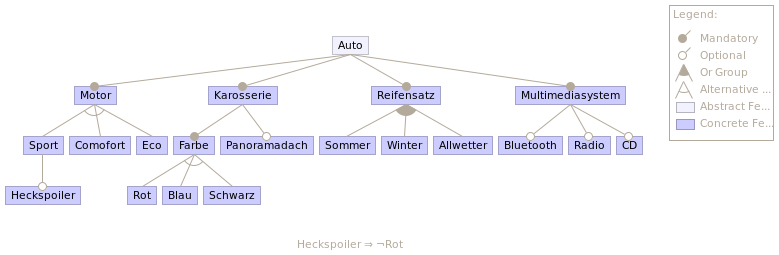
\includegraphics[width=\linewidth]{assets/Variantenmanagement}
                \end{centering}
            \pagebreak
            \item
                \fboxsep0.1mm
\noindent
\unfold\blank\myPlus Auto\\
\tab\unfold\mandatory\myPlus Motor\\
\tab\tab\unfold\Alternative\myPlusblank Sport\\
\tab\tab\tab\nofold\optional\myBox Heckspoiler\\
\tab\tab\nofold\Alternative\myMinus Comofort\\
\tab\tab\nofold\Alternative\myMinus Eco\\
\tab\unfold\mandatory\myPlus Karosserie\\
\tab\tab\unfold\mandatory\myPlus Farbe\\
\tab\tab\tab\nofold\Alternative\myMinus Rot\\
\tab\tab\tab\nofold\Alternative\myPlusblank Blau\\
\tab\tab\tab\nofold\Alternative\myMinus Schwarz\\
\tab\tab\nofold\optional\myBox Panoramadach\\
\tab\unfold\mandatory\myPlus Reifensatz\\
\tab\tab\nofold\myOr\myPlusblank Sommer\\
\tab\tab\nofold\myOr\myPlusblank Winter\\
\tab\tab\nofold\myOr\myBox Allwetter\\
\tab\unfold\mandatory\myPlus Multimediasystem\\
\tab\tab\nofold\optional\myBox Bluetooth\\
\tab\tab\nofold\optional\myPlusblank Radio\\
\tab\tab\nofold\optional\myBox CD\\


                \fboxsep0.1mm
\noindent
\unfold\blank\myPlus Auto\\
\tab\unfold\mandatory\myPlus Motor\\
\tab\tab\unfold\Alternative\myMinus Sport\\
\tab\tab\tab\nofold\optional\myMinus Heckspoiler\\
\tab\tab\nofold\Alternative\myPlusblank Comofort\\
\tab\tab\nofold\Alternative\myMinus Eco\\
\tab\unfold\mandatory\myPlus Karosserie\\
\tab\tab\unfold\mandatory\myPlus Farbe\\
\tab\tab\tab\nofold\Alternative\myPlusblank Rot\\
\tab\tab\tab\nofold\Alternative\myMinus Blau\\
\tab\tab\tab\nofold\Alternative\myMinus Schwarz\\
\tab\tab\nofold\optional\myBox Panoramadach\\
\tab\unfold\mandatory\myPlus Reifensatz\\
\tab\tab\nofold\myOr\myPlusblank Sommer\\
\tab\tab\nofold\myOr\myBox Winter\\
\tab\tab\nofold\myOr\myBox Allwetter\\
\tab\unfold\mandatory\myPlus Multimediasystem\\
\tab\tab\nofold\optional\myBox Bluetooth\\
\tab\tab\nofold\optional\myBox Radio\\
\tab\tab\nofold\optional\myBox CD\\

        \end{enumerate}
\end{document}
